\documentclass{classrep}
\usepackage[utf8]{inputenc}
\frenchspacing

\usepackage{graphicx}
\usepackage[usenames,dvipsnames]{color}
\usepackage[hidelinks]{hyperref}
\usepackage[section]{placeins}
\usepackage{float}
\usepackage{amsmath, amssymb, mathtools}

\setlength{\abovecaptionskip}{0pt}
\setlength{\belowcaptionskip}{0pt}

\usepackage{fancyhdr, lastpage}
\pagestyle{fancyplain}
\fancyhf{}
\renewcommand{\headrulewidth}{0pt}
\cfoot{\thepage\ / \pageref*{LastPage}}


\studycycle{Informatyka, studia dzienne, I st.}
\coursesemester{IV}

\coursename{Inteligentna Analiza Danych}
\courseyear{2017/2018}

\courseteacher{mgr inż. Paweł Tarasiuk}
\coursegroup{piątek, 10:15}

\author{%
  \studentinfo[215145@edu.p.lodz.pl]{Michał Chudzik}{215145}\\
  \studentinfo[210320@edu.p.lodz.pl]{Michał Sobczyk}{210320}%
}

\title{Zadanie 1}

\begin{document}
\maketitle
\thispagestyle{fancyplain}

\section{Cel}
	Celem zadania jest implementacja i zbadania sieci neuronowej. Implementacja składa się ze skalowalnej sieci neuronowej wykorzystującej wsteczną propagację błędów jako metodę nauki oraz momentum.

\section{Wprowadzenie}
	\textbf{Perceptron wielowarstwowy}-  głównym elementem są neurony przetwarzające. Każdy neuron posiada dowolną liczbę wejść oraz jedno wyjście. Neurony są pogrupowane w warstwy, gdzie każde dwie sąsiednie warstwy są połączone iloczynem kartezjańskim. Na wejście neuronu trafiają wyjścia wszystkich neuronów z warstwy poprzedniej.


Przetwarzanie wymaga obliczonych wcześniej wartości wyjściowych z poprzednich warstw. Ten proces dany jest poniższym wzorem
\begin{equation} \label{eq:feedforward}
	a_{t+1} = \sigma ( Wa_t + b),
\end{equation}
gdzie $a_{t+1}$ jest macierzą wyjścia warstwy neuronowej, $a_t$ macierzą wejścia warstwy neuronowej, W macierzą wag, b macierzą biasów a $\sigma$ jest funkcją aktywacji daną wzorem
\begin{equation} \label{eq:activation}
	\sigma = \frac{1}{1 + e^{-x}}.
\end{equation}


Proces nauki jest wykonany za pomocą metody najmniejszych spadków. Aktualizacja wag dana jest wzorem
\begin{equation} \label{eq:generalBackPropagationWeight}
	w_i = w_i - \lambda \cdot \frac{\delta E}{\delta w_i},
\end{equation}
gdzie $w_i$ jest wagą która jest aktualizowana, $\lambda$ współczynnik uczenia, $E_{total}$ dany jest wzorem
\begin{equation} \label{eq:totalError}
	E = \sum \frac{1}{2}(target - output)^2,
\end{equation}
gdzie output oznacza wynik końcowy sieci neuronowej a target oczekiwaną wartość tegoż wyniku.


Aktualizacja biasów zachodzi w sposób
\begin{equation} \label{eq:generalBackPropagationBias}
	b_i = b_i - \lambda \cdot \frac{\delta E}{\delta b_i},
\end{equation}
gdzie $b_i$ jest zmienianym biasem.

\section{Opis implementacji}
Aplikacja została stworzona w języku Python3 przy użyciu dodatkowych modułów bibliotecznych takich jak:
		\begin{itemize}
			\item matplotlib - generowanie wykresów
			\item sklearn - import wybranych zbiorów danych
		\end{itemize}

\section{Materiały i metody}
Analiza danych została przeprowadzona na zbiorze opisującym wina irysy \cite{irisdataset}


Eksperymenty 1 - 3 zostały przeprowadzone za pomocą sieci neuronowej dla zbioru Iris. Zasób treningowy liczył 100 losowych krotek, a reszta (40) została użyta do przetestowania klasyfikacji. Dla omawianych eksperymentów algorytm wykonywał 1000 iteracji.\\


\textbf{Eksperyment 1 - Zbiór irysów}\\
		Wpływ ilości neuronów na uczenie.\\
		learning rate = 0.5\\
		momentum = 0.0\\
		size - rozłożenie neuronów
		\begin{itemize}
			\item \textbf{E1.1}
			 size = [4, 2, 3]
			\item \textbf{E1.2} 
			size = [4, 7, 3]
			\item \textbf{E1.3}
			size = [4, 12, 3]
			\item \textbf{E1.4}
			size = [4, 20, 3]
		\end{itemize}
	
	\textbf{Eksperyment 2 - Zbiór irisów}\\
		Wpływ learning rate na uczenie.\\
		size = [4, 2, 3]\\
		momentum =  0.0
		\begin{itemize}
			\item \textbf{E2.1}
			 learning rate = 0.2
			\item \textbf{E2.2} 
			learning rate = 0.4
			\item \textbf{E2.3}
			learning rate = 0.6
			\item \textbf{E2.4}
			learning rate = 0.8
		\end{itemize}
	
	\textbf{Eksperyment 3 - Zbiór irysów}\\
		Wpływ wartości momentum na uczenie.\\
		size = [4, 2, 3]\\
		learning rate = 0.2
		\begin{itemize}
			\item \textbf{E3.1}
			 momentum = 0.3
			\item \textbf{E3.2} 
			momentum = 0.5
			\item \textbf{E3.3}
			momentum = 0.7
			\item \textbf{E3.4}
			momentum = 0.9
		\end{itemize}


\section{Wyniki}

\subsection{Eksperyment 1}
		\begin{figure}[H]
			\begin{minipage}{0.5\linewidth}
				\centering
				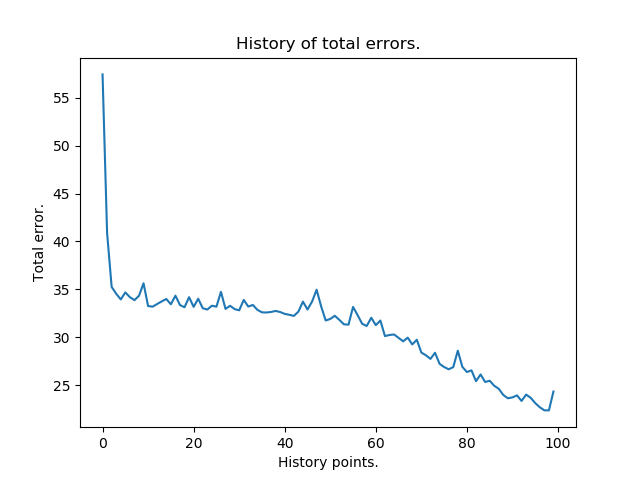
\includegraphics[scale=0.25]{iris_nn_s2.png}
				\caption{E1.1 Test rate  0.78}
			\end{minipage}
			\begin{minipage}{0.5\linewidth}
				\centering
				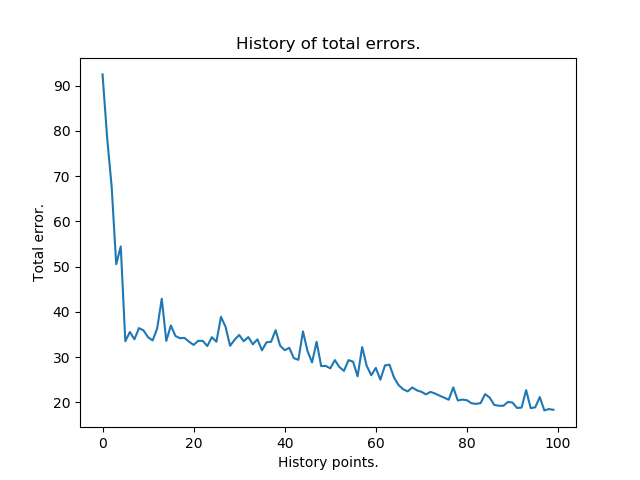
\includegraphics[scale=0.25]{iris_nn_s7.png}
				\caption{E1.2 Test rate  0.82}
				\label{E1.2}
			\end{minipage}
			\begin{minipage}{0.5\linewidth}
				\centering
				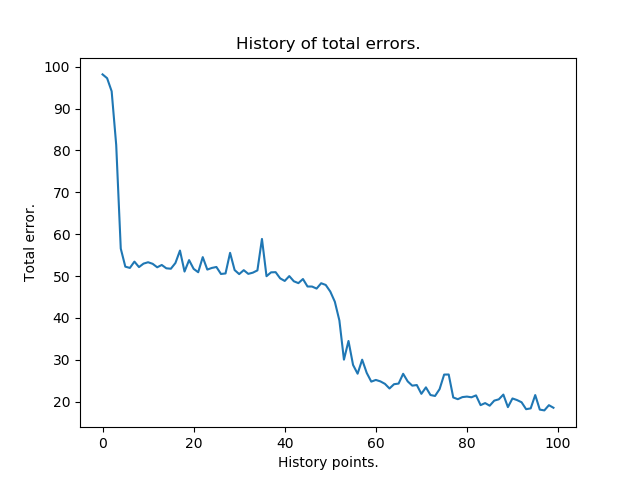
\includegraphics[scale=0.25]{iris_nn_s12.png}
				\caption{E1.3 Test rate  0.78}
			\end{minipage}
			\begin{minipage}{0.5\linewidth}
				\centering
				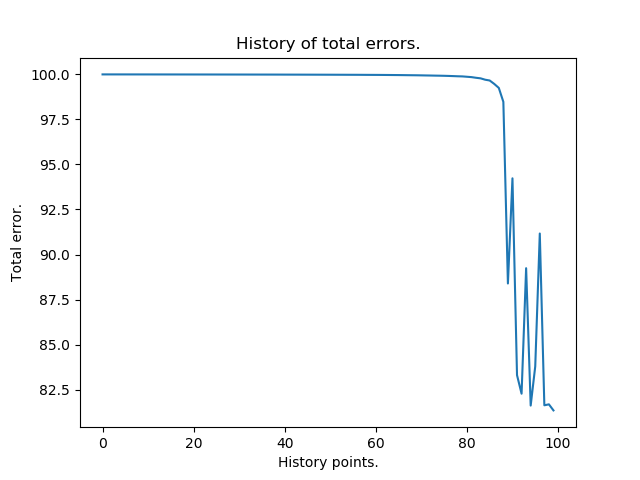
\includegraphics[scale=0.25]{iris_nn_s20.png}
				\caption{E1.4 Test rate  0.42}
			\end{minipage}
		\end{figure}
		\FloatBarrier
	\subsection{Eksperyment 2}
		\begin{figure}[H]
			\begin{minipage}{0.5\linewidth}
				\centering
				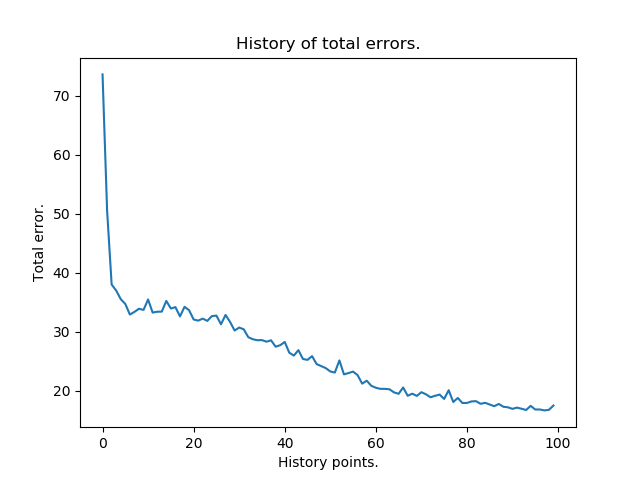
\includegraphics[scale=0.25]{iris_nn_l2.png}
				\caption{E2.1 Test rate  0.3}
			\end{minipage}
			\begin{minipage}{0.5\linewidth}
				\centering
				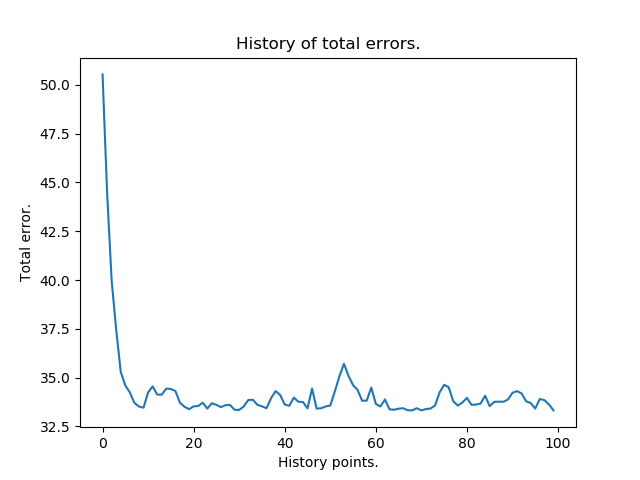
\includegraphics[scale=0.25]{iris_nn_l4.png}
				\caption{E2.2 Test rate  0.7}
				\label{E2.2}
			\end{minipage}
			\begin{minipage}{0.5\linewidth}
				\centering
				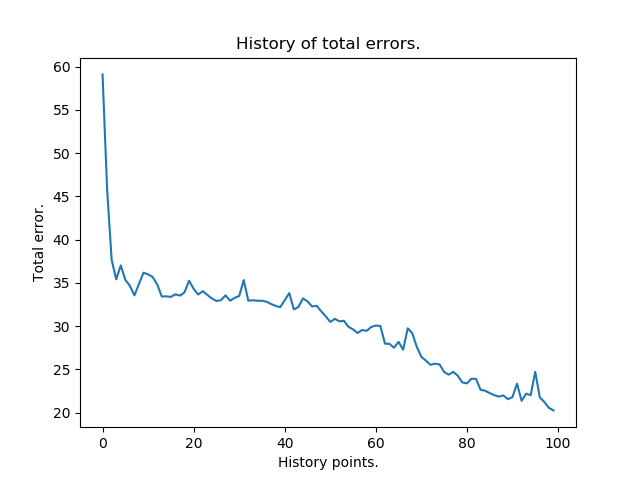
\includegraphics[scale=0.25]{iris_nn_l6.png}
				\caption{E2.3 Test rate  0.7}
			\end{minipage}
			\begin{minipage}{0.5\linewidth}
				\centering
				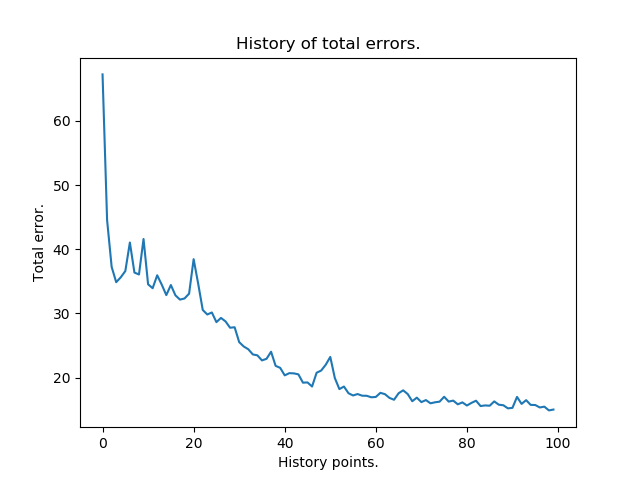
\includegraphics[scale=0.25]{iris_nn_l8.png}
				\caption{E2.4 Test rate  0.64}
			\end{minipage}
		\end{figure}
		\FloatBarrier
	\subsection{Eksperyment 3}
		\begin{figure}[H]
			\begin{minipage}{0.5\linewidth}
				\centering
				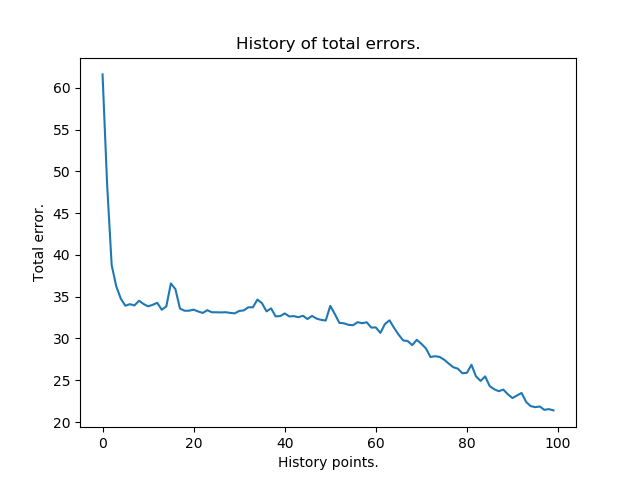
\includegraphics[scale=0.25]{iris_nn_m3.png}
				\caption{E3.1 Test rate  0.64}
			\end{minipage}
			\begin{minipage}{0.5\linewidth}
				\centering
				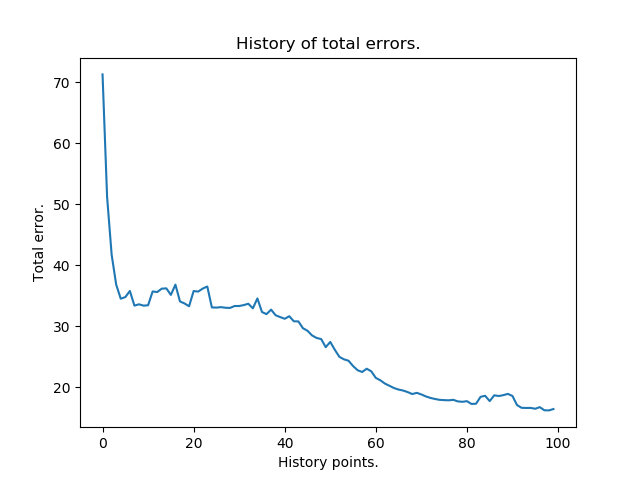
\includegraphics[scale=0.25]{iris_nn_m5.png}
				\caption{E3.2 Test rate  0.92}
				\label{E3.2}
			\end{minipage}
			\begin{minipage}{0.5\linewidth}
				\centering
				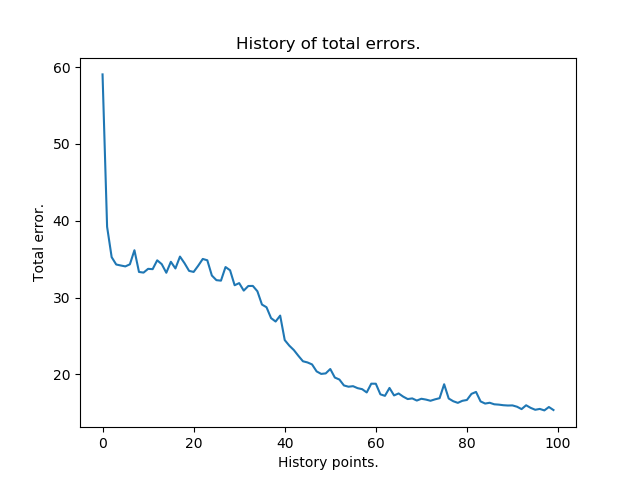
\includegraphics[scale=0.25]{iris_nn_m7.png}
				\caption{E3.3 Test rate  0.9}
				\label{E3.3}
			\end{minipage}
			\begin{minipage}{0.5\linewidth}
				\centering
				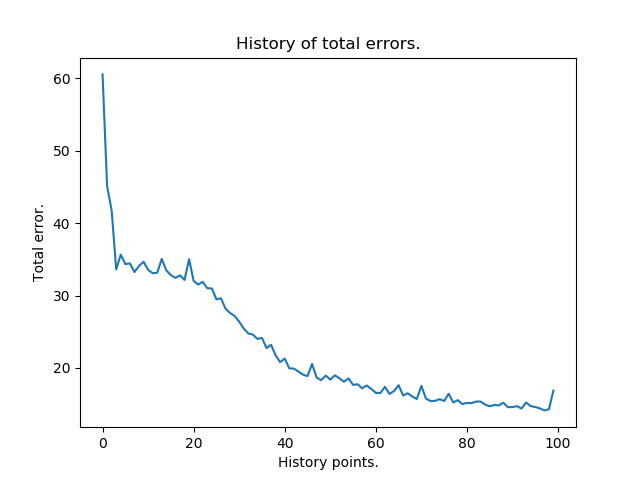
\includegraphics[scale=0.25]{iris_nn_m9.png}
				\caption{E3.4 Test rate  0.74}
				\label{E3.4}
			\end{minipage}
		\end{figure}
		\FloatBarrier
			

\section{Dyskusja}

\section{Wnioski}


\begin{thebibliography}{0}
\bibitem{irisdataset}https://archive.ics.uci.edu/ml/datasets/iris
Zbiór danych dla irysów
\bibitem{backPopgation}https://mattmazur.com/2015/03/17/a-step-by-step-backpropagation-example/
Back Propagation
\end{thebibliography}

\end{document}